\documentclass[12pt,a4paper]{article}
\usepackage[utf8]{inputenc}
\usepackage{geometry}
\geometry{a4paper, margin=1in}
\usepackage{titlesec}
\usepackage{hyperref}
\usepackage{cite}
\usepackage{listings}
\usepackage{graphicx}

\begin{document}

\begin{titlepage}
    \centering
    \vspace*{1cm}
    
    {\Large \textbf{Ecogent: A Local-First Multi-Agent Architecture for Reducing LLM Costs Through Persistent Tools and Adaptive Model Routing}} \\
    
    \vspace{1.5cm}
    {\large \textbf{Report on Thesis Proposal}} \\
    
    \vspace{2cm}
    
    \textbf{Course No.} -- CSE 061 4100 \\
    \textbf{Course Title} -- Project and Thesis - 1 \\

    \vspace{1.5cm}

    {\Large \textbf{Submitted By:}} \\
        \vspace{0.5cm}
    \textbf{Name:} Samrat Biswas \\
    \vspace{0.3cm}
    \textbf{Student ID:} 10023105101003 \\
    \vspace{0.3cm}
    \textbf{Department:} Computer Science \& Engineering \\
    \vspace{0.3cm}
    \textbf{Year:} 4th Year, 1st Semester

    
    \vfill
\end{titlepage}

\begin{abstract}
\noindent Large Language Model (LLM)-based agents have strong capabilities in autonomous task execution across domains such as software engineering, browser automation, and system operations. However, existing agent architectures suffer from inefficient memory utilization, high token cost, and a lack of structured execution control. This research proposes \textbf{Ecogent} (Economical Cognitive Agent), a Workflow-Driven, Local-First Multi-Agent Architecture that integrates structured workflow representations, semantic memory retrieval using Chroma DB, and dynamic tool selection. The system distributes tasks across main and sub-workflows, represented as JSON, while storing compressed semantic keys in a vector database for efficient retrieval. A lightweight local NLP+ML supervisor model orchestrates task routing among specialized agents (coding, browser, testing, and OS), falling back to a local tiny deep learning model and only invoking cloud LLMs as a last resort. Experimental design suggests that this architecture significantly reduces redundant reasoning, lowers cloud API costs, and improves execution efficiency compared to traditional monolithic, cloud-native agent systems.
\end{abstract}

\section{Introduction}
Nowadays LLMs are not only for chatting or getting personalized information; when AI Agents come into the picture, it has also changed the world. People can use AI as an assistant for different kinds of tasks, for example, Software development, Software Testing, Browser Automation, Data mining, or analysis, like a human. These tasks are performed by an AI agent, which acts like the ``hands'' of the LLM to control user systems. However, current agent systems are still inefficient, not well-optimized, and high-cost.

\section{Motivation}
Current AI agents often behave like general-purpose systems. They try to handle all types of tasks without proper structure. This creates several problems:
\begin{itemize}
    \item High token usage due to full chat history
    \item Repeated reasoning for similar tasks
    \item Poor memory reuse
    \item Lack of clear workflow structure
    \item No local supervisor to control the Agent to efficiently deal with an LLM
\end{itemize}

\noindent From a system design perspective, this is inefficient. Instead of storing full conversations, it is more effective to store meaningful workflow steps and reusable knowledge. Also, current Agents don't use any local Intelligence supervisor. This research is motivated by the idea that:
\textit{``Agents should not remember everything; they should remember what matters. Also, found that many people are suffering a huge amount of AI Credit loss when they are using an AI Assistant for daily tasks.''}

\section{Problem Statement}
Existing LLM-based agent systems face the following problems:
\begin{itemize}
    \item \textbf{Unstructured Memory Usage:} Most agents store full chat history, which increases token cost and reduces efficiency.
    \item \textbf{Lack of Workflow Representation:} Tasks are executed without structured planning, making debugging and optimization difficult.
    \item \textbf{Inefficient Tool Selection:} Tools are often selected without semantic understanding, leading to incorrect or repeated actions.
    \item \textbf{Limited Knowledge Reuse:} Previous workflows are not reused effectively, causing redundant computation.
    \item \textbf{Absence of a Local Supervisor:} The AI Agent only works with some logic based on LLM output, so sometimes it uses an extra API call to understand the proper task.
\end{itemize}

\section{Research Objectives}
The main objectives of this research are to overcome the limitations of current cloud-native systems (like Claude Code and Google Antigravity) and introduce better token economics \cite{token_economics, ai_tokenomics}:
\begin{itemize}
    \item \textbf{Stop sending huge context windows:} Eliminate the dependency on massive context windows by retaining only what matters, aligning with marginal token allocation \cite{marginal_token}.
    \item \textbf{Stop using LLM code generation each time:} Avoid generating unique, disposable code loops for every task \cite{claude_code_dive}. Instead, reuse persistent, pre-made local tools.
    \item \textbf{Keep a proper plan in a JSON:} Move away from unstructured natural language plans. Generate deterministic JSON roadmaps containing full task steps.
    \item \textbf{Stop communicating with the LLM for small or existing tasks:} Reduce network bandwidth and runtime costs by handling minor navigations and interactions locally \cite{efficient_agents}.
    \item \textbf{Stop sending text-based skills to the LLM:} Avoid passing lengthy text descriptions of Model Context Protocol (MCP) servers or tools directly into the main prompt.
\end{itemize}

\section{Research Questions}
This research aims to answer the following questions:
\begin{enumerate}
    \item \textbf{RQ1:} How much does a multi-tier local-first routing strategy (NLP supervisor $\rightarrow$ tiny model $\rightarrow$ cloud LLM) reduce cloud API token usage compared to single-tier cloud-native agent systems?
    \item \textbf{RQ2:} Can structured JSON workflow representations combined with semantic memory (Chroma DB) improve task execution efficiency and reduce redundant reasoning in multi-agent systems?
    \item \textbf{RQ3:} To what extent does persistent, pre-made tool reuse decrease operational cost and execution latency compared to ephemeral, LLM-generated scripts?
    \item \textbf{RQ4:} How effectively can a local NLP+ML-based supervisor select appropriate tools and route tasks without invoking a cloud LLM?
\end{enumerate}

\section{Related Works / Literature Review}
Recent research in AI agents has focused on improving reasoning, architecture, and token economics. Surveys on emerging AI agent architectures for reasoning, planning, and tool calling \cite{agent_survey} highlight the shift towards more structured agentic workflows. For example, AutoGPT+P \cite{autogpt_p} explores affordance-based task planning with LLMs to improve execution reliability.

\medskip

\noindent Furthermore, toolchains for end-to-end orchestration such as LangChain, LangGraph, and LangSmith have been rigorously analyzed to provide structured execution graphs for agents \cite{langchain_langgraph}. However, most cloud-native systems, including Claude Code \cite{claude_code_dive}, heavily rely on massive context windows and real-time ephemeral code generation, which significantly impacts their token economy and cost-efficiency.

\medskip

\noindent To address cost-efficiency, various studies have proposed frameworks focusing on agent token economics \cite{token_economics} and pricing models in foundation models \cite{ai_tokenomics}, emphasizing that agentic systems should be designed as marginal token allocators \cite{marginal_token} to build effective agents while reducing costs \cite{efficient_agents}. 

\medskip

\noindent In the realm of workflow optimization, automated machine learning (AutoML) libraries like FLAML \cite{flaml} provide fast and lightweight capabilities that can be integrated into cost-aware automation pipelines \cite{cost_aware_automl}. Finally, managing agent memory effectively requires robust vector databases; performance analyses of databases like Chroma, Qdrant, and FAISS \cite{chroma_faiss_analysis} are critical in selecting the right local storage medium for semantic tool retrieval.

\subsection{Research Gap}
Despite these advances, current systems still lack:
\begin{itemize}
    \item Structured workflow memory with lightweight semantic tool tracking.
    \item Efficient reuse of past executions via persistent local schemas.
    \item Cost-aware multi-agent orchestration balancing local ML supervisors and cloud LLMs.
    \item A multi-tier triage mechanism that routes tasks through local NLP, a local tiny model, and a cloud fallback sequentially.
\end{itemize}
This research aims to bridge these gaps by proposing the Ecogent architecture.

\section{Proposed Methodology: Ecogent Architecture}
This research proposes a hybrid system combining structured workflows, semantic memory, and multi-agent execution, heavily prioritizing local computation.

\subsection{Key Agent Features}
The proposed agent architecture includes the following core features:
\begin{enumerate}
    \item Local Vector DB (Chroma) for storing semantic keys.
    \item FLAML integration for lightweight automated machine learning (AutoML) tasks.
    \item Common tools and OS/IO functions are pre-made and kept in a fixed local database so they are never deleted.
    \item Dynamic creation of new tools via LLM when needed, storing their references in the Vector DB based on the project.
    \item Tools are stored as JSON schemas, with their natural name keys addressed in the Vector DB for easy natural language matching.
    \item A local NLP + ML-based supervisor decides the best tools to select or create.
    \item Fallback to a local tiny deep learning model if the supervisor cannot find a solution, minimizing cloud API calls.
    \item Only if the tiny model fails does the system communicate with a cloud LLM (via LangChain/LangGraph) to handle complex situations or create new tools.
    \item Creation of a JSON tree for the action plan upon receiving the first prompt or creating a project. The tree provides a clear view for verification.
    \item The Project JSON tree can be dynamically healed or updated by the LLM later based on the task progress.
    \item Dedicated browser support for local testing and UI evaluation.
\end{enumerate}

\subsection{System Architecture}
\begin{verbatim}
User Input -> NLP+ML Supervisor -> Tiny Model -> Cloud LLM
                |                      |
                +-> Workflow JSON (Main + Sub)
                +-> Local Tools (Pre-made)
                +-> Vector Memory (Chroma DB)
                +-> Multi-Agent Execution
\end{verbatim}

\subsection{Architectural Comparison: Ecogent vs. Cloud-Native}

\begin{figure}[htbp]
    \centering
    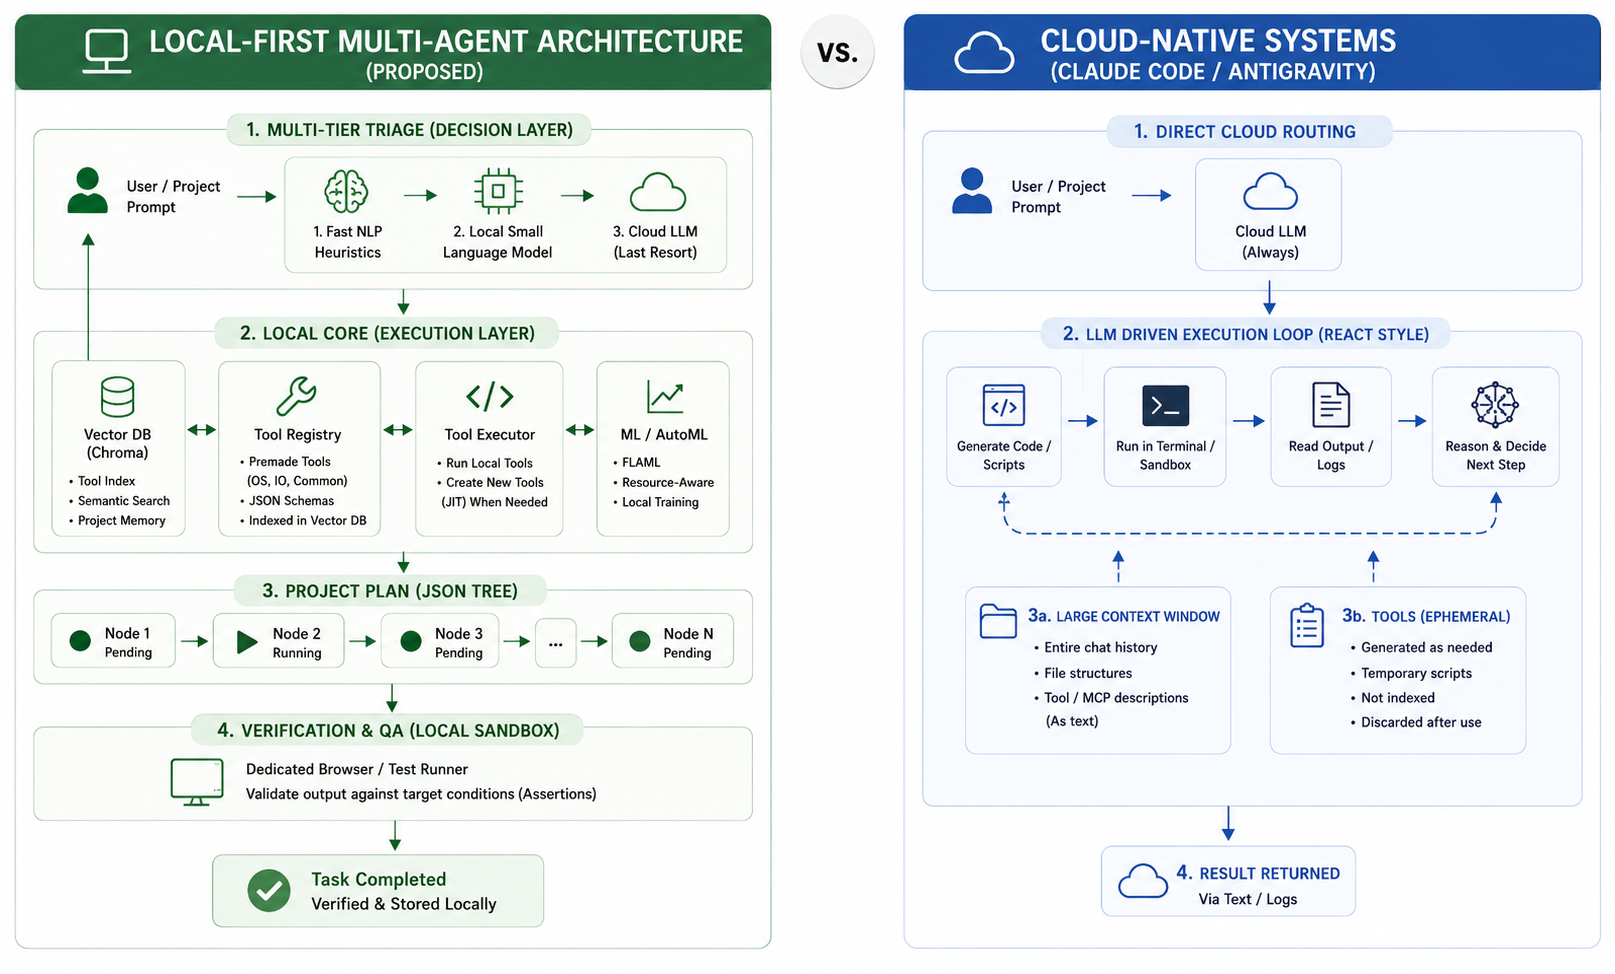
\includegraphics[width=0.8\linewidth]{compare.png}
    \caption{Comparison of Ecogent's local-first architecture vs. cloud-native agent systems, illustrating the key structural differences in task routing, tool management, and memory handling.}
    \label{fig:architecture_comparison}
\end{figure}

\subsection{Workflow Representation}
Tasks are distributed across main and sub-workflows, heavily structured in JSON to maintain a clear, verifiable action plan.

\begin{table}[htbp]
\centering
\resizebox{\textwidth}{!}{%
\begin{tabular}{|p{0.25\linewidth}|p{0.35\linewidth}|p{0.35\linewidth}|}
\hline
\textbf{Dimension} & \textbf{Proposed Local-First (Ecogent)} & \textbf{Cloud-Native (e.g., Claude Code, Antigravity)} \\ \hline
\textbf{System Paradigm} & Decentralized Local Cache: Prioritizes local computation; cloud is a premium last resort. & Monolithic Cloud Shell: Offloads cognitive planning to cloud models. \\ \hline
\textbf{Multi-Agent Topology} & Hierarchical State Isolation: Specialized sub-agents write to isolated nodes in a shared JSON tree. & Unitary Sequential Loops: Rely on a single chat thread that bloats context string. \\ \hline
\textbf{Orchestration \& Triage} & Multi-Tier Hierarchical Triage: Sequential routing utilizing fast NLP, a local tiny model, and a cloud fallback. & Single-Tier Direct Ingestion: Routes raw natural language payloads directly to high-parameter cloud models. \\ \hline
\textbf{Tool Registry} & Deterministic Persistent Indexing: Tool definitions are systematically indexed in a local Vector DB (Chroma). & Imperative Ephemeral Scripting: Generates transient scripts directly in terminal sandboxes that are discarded. \\ \hline
\textbf{Extensibility Mechanics} & Just-in-Time Tool Generation: Dynamically writes missing capabilities via an LLM tool call, persisting the reference schema locally with semantic identifiers. & Context-Bound Synthesis: Automatically compiles situational code snippets within the active prompt window without indexing for global reuse. \\ \hline
\textbf{Verification \& QA} & Dedicated Sandbox Evaluation: Integrates a local browser loop to assert UI render states against JSON. & Textual Console Analysis: Evaluates output by piping stdout/stderr back into the LLM context. \\ \hline
\textbf{Algorithmic Planning} & Structured Declarative Execution: Generates deterministic JSON roadmaps containing full task steps. & Autoregressive Feedback Loops: Fluid ReAct frameworks evaluating stdout streams in real time. \\ \hline
\textbf{Statistical Optimization} & Resource-Aware Local AutoML: Deploys lightweight automated machine learning (FLAML) optimized for strict hardware, RAM, and time boundaries. & Distributed Enterprise Scaling: Relies on commercial cloud APIs, unconstrained resource scaling, or unoptimized custom Python code. \\ \hline
\textbf{Security \& Data} & Strict Local Containment: Code, metadata, and database schemas remain localized. & Continuous Perimeter Streaming: Streams operational source code and vectors to third-party endpoints. \\ \hline
\textbf{Computational Overhead} & Frugal Resource Allocation: Maximizes system idle states to preserve battery and token budgets. & High Intermittent Saturation: Requires stable connections and generates significant per-session overhead. \\ \hline
\end{tabular}%
}
\caption{Comparison of Ecogent vs Cloud-Native Architectures}
\label{tab:architecture_comparison}
\end{table}


\noindent\begin{minipage}{\textwidth}
\textbf{Example Project JSON Plan:}
\begin{lstlisting}[basicstyle=\footnotesize\ttfamily]
{
  "project_id": "proj_001",
  "project_name": "Customer Segmentation Engine",
  "global_status": {
    "how_much_filled_percentage": 0.0,
    "current_active_node": "node_data_ingest"
  },
  "project_tree": [
    {
      "node_id": "node_data_ingest",
      "task_title": "Load and Verify Client CSV",
      "execution_tier": "local_premade_io",
      "reasoning": "System requires raw structural inputs
          verified locally before kicking off the FLAML
          search pipeline.",
      "status": "pending",
      "how_much_filled_node": 0.0,
      "target_conditions": [
        {
          "assertion_type": "FILE_EXISTS",
          "target": "./data/clients.csv",
          "error_msg": "Source clients.csv file is missing
              from local project directory."
        },
        {
          "assertion_type": "FILE_MIN_SIZE_KB",
          "target": 10,
          "error_msg": "The target clients.csv data file
              is corrupted or contains empty content."
        }
      ]
    },
    {
      "node_id": "node_automl_train",
      "task_title": "Run FLAML Cluster Optimization",
      "execution_tier": "local_flaml_automl",
      "reasoning": "Train local clustering algorithms to
          identify optimal consumer segments based on
          localized numerical vectors.",
      "status": "pending",
      "how_much_filled_node": 0.0,
      "target_conditions": [
        {
          "assertion_type": "FILE_EXISTS",
          "target": "./models/cluster_pipeline.pkl",
          "error_msg": "FLAML optimization pipeline failed
              to compile or save trained model file."
        },
        {
          "assertion_type": "CSV_COLUMN_EXISTS",
          "target": {
            "file_path": "./data/output_segments.csv",
            "column_name": "cluster_id"
          },
          "error_msg": "The predictive model failed to
              append cluster labels to output dataframe."
        }
      ]
    }
  ]
}
\end{lstlisting}
\end{minipage}

\subsection{Semantic Memory (Chroma DB)}
Instead of storing the full chat, the system extracts workflow keys:

\textbf{Example:}
\begin{itemize}
    \item login\_auth\_fix
    \item checkout\_payment\_error
\end{itemize}
These natural name keys are stored in Chroma DB and used to retrieve similar workflows or tools.

\subsection{Multi-Agent System}
The system includes specialized agents:
\begin{itemize}
    \item \textbf{Coding Agent} $\rightarrow$ handles programming tasks
    \item \textbf{Browser Agent} $\rightarrow$ handles web automation (dedicated browser support)
    \item \textbf{Testing Agent} $\rightarrow$ validates and debugs
    \item \textbf{OS Agent} $\rightarrow$ handles system-level operations
\end{itemize}

A local NLP + ML-based supervisor (with a local tiny deep learning model fallback) decides which agent to use before invoking the cloud LLM.

\subsection{Multi-Tier Routing Pseudocode}
The following pseudocode illustrates the multi-tier triage logic of the Ecogent supervisor:

\begin{lstlisting}[language=Python, basicstyle=\footnotesize\ttfamily]
def ecogent_route(user_input):
    # Tier 1: Fast NLP + ML-based local supervisor
    intent, confidence = nlp_ml_supervisor.classify(user_input)
    if confidence >= THRESHOLD_HIGH:
        tool = vector_db.retrieve_tool(intent)
        if tool:
            return execute_local(tool, user_input)

    # Tier 2: Local tiny deep learning model fallback
    result = tiny_local_model.infer(user_input)
    if result.is_resolved:
        return result.output

    # Tier 3: Cloud LLM via LangGraph (last resort)
    json_plan = cloud_llm.generate_plan(user_input)
    store_workflow(json_plan)
    return execute_plan(json_plan)
\end{lstlisting}

\subsection{Tool System}
The system includes:
\begin{itemize}
    \item Pre-made built-in tools (kept permanently in the local database)
    \item LLM-generated tools (created dynamically, validated, and stored)
\end{itemize}
Tools are stored with semantic descriptions in JSON schemas and retrieved using Chroma DB.

\subsection{Execution Flow}
\begin{verbatim}
Input -> NLP Supervisor -> Tiny Model Check -> Cloud LLM (if complex)
      -> Retrieve Memory -> Select Agent
      -> Execute Tool -> Update JSON Workflow -> Store Key
\end{verbatim}

\section{Expected Outcomes}
The expected outcomes of this research are:
\begin{itemize}
    \item Eliminates unnecessary massive context window processing
    \item Drastically reduces cloud API token usage and latency
    \item Improves task execution speed with deterministic JSON plans
    \item Reuses previous workflows and local tools effectively
    \item Provides better control over agent behavior and hardware resource constraints
\end{itemize}

\section{Conclusion}
This research proposes Ecogent, a workflow-driven, local-first multi-agent system design that improves efficiency by combining structured JSON workflows, semantic memory, pre-made persistent tools, and specialized agents.

\medskip

\noindent By introducing a multi-tier triage mechanism that sequentially routes tasks through a local NLP+ML supervisor, a local tiny deep learning model, and a cloud LLM as a last resort, Ecogent addresses the key inefficiencies of current cloud-native agent systems. This approach can be used in real-world applications such as software automation, testing systems, and intelligent assistants for general purposes.

\begin{thebibliography}{99}

\bibitem{token_economics}
Y. Chen, J. Chen, C. He, Y. Li, Y. Ji, Y. Wu, D. Yang, L. Diao, L. Shou, H. Zhang, H. Li, and G. Chen, ``Token Economics for LLM Agents: A Dual-View Study from Computing and Economics.'' \textit{arXiv preprint arXiv:2605.09104}, 2025.

\bibitem{ai_tokenomics}
Q. Zhu, ``AI Tokenomics: The Economics of Tokens, Computation, and Pricing in Foundation Models.'' \textit{arXiv preprint arXiv:2606.24616}, 2026.

\bibitem{marginal_token}
S. Zhu, ``Agentic AI Systems Should Be Designed as Marginal Token Allocators.'' \textit{arXiv preprint arXiv:2605.01214}, 2025.

\bibitem{claude_code_dive}
J. Liu, X. Zhao, X. Shang, and Z. Shen, ``Dive into Claude Code: The Design Space of Today's and Future AI Agent Systems.'' \textit{arXiv preprint arXiv:2604.14228}, 2025.

\bibitem{efficient_agents}
N. Wang, X. Hu, P. Liu, H. Zhu, Y. Hou, H. Huang, S. Zhang, J. Yang, J. Liu, G. Zhang, C. Zhang, J. Wang, Y.~E. Jiang, and W. Zhou, ``Efficient Agents: Building Effective Agents While Reducing Cost.'' \textit{arXiv preprint arXiv:2508.02694}, 2025.

\bibitem{agent_survey}
T. Masterman, S. Besen, M. Sawtell, and A. Chao, ``The Landscape of Emerging AI Agent Architectures for Reasoning, Planning, and Tool Calling: A Survey.'' \textit{arXiv preprint arXiv:2404.11584}, 2024.

\bibitem{autogpt_p}
T. Birr, C. Pohl, A. Younes, and T. Asfour, ``AutoGPT+P: Affordance-based Task Planning with Large Language Models.'' \textit{arXiv preprint arXiv:2402.10778}, 2024.

\bibitem{langchain_langgraph}
R. Sapkota, R. Shrestha, M. Rijal, and M. Karkee, ``LangChain vs. LangGraph vs. LangSmith: Taxonomies of Agentic AI Toolchains for End-to-End Orchestration.'' \textit{TechRxiv}, 2025.

\bibitem{flaml}
C. Wang, Q. Wu, M. Weimer, and E. Zhu, ``FLAML: A Fast and Lightweight AutoML Library.'' \textit{MLSys}, 2021.

\bibitem{cost_aware_automl}
A. Sindhu and S. Arumugam, ``Agent-Based Generative AI Model for Cost-Aware Automation in Machine Learning Pipelines.'' \textit{IEEE Access}, vol.~13, 2025.

\bibitem{chroma_faiss_analysis}
E. \"{O}zt\"{u}rk and A. Mesut, ``Performance Analysis of Chroma, Qdrant, and FAISS Databases.'' \textit{UNITECH -- Selected Papers}, 2024.

\end{thebibliography}

\end{document}
